\documentclass[11pt,a4paper]{article}
\usepackage[utf8]{inputenc}
\usepackage[T1]{fontenc}
\usepackage[spanish]{babel}
\usepackage{lmodern}
\usepackage[left=2cm,right=2cm,top=2cm,bottom=2cm]{geometry}
\usepackage{graphicx}
\usepackage{xcolor}
\usepackage{enumitem}
\usepackage{titlesec}
\titlespacing*{\section}{0pt}{16pt}{8pt}
\titleformat{\section}{\large\bfseries\color{isa}}{}{0pt}{}
\usepackage[hidelinks]{hyperref}
\definecolor{isa}{RGB}{0,70,130}
\setlength{\parindent}{0pt}
\setlength{\parskip}{7pt}
\linespread{1.06}
\setlist[enumerate]{leftmargin=*,itemsep=8pt,topsep=6pt}
\setlist[itemize]{leftmargin=*,itemsep=2pt,topsep=3pt}
\begin{document}
\sloppy
\noindent\begin{minipage}[c]{0.76\linewidth}
{\LARGE\bfseries\color{isa} Instalación del firmware}\par
{\large Arduino UNO · Equipo de control de motor CC}\par
{\small ISA · Universidad de Sevilla\\\href{mailto:ialvarado@us.es}{ialvarado@us.es}}
\end{minipage}\hfill
\begin{minipage}[c]{0.22\linewidth}
\centering
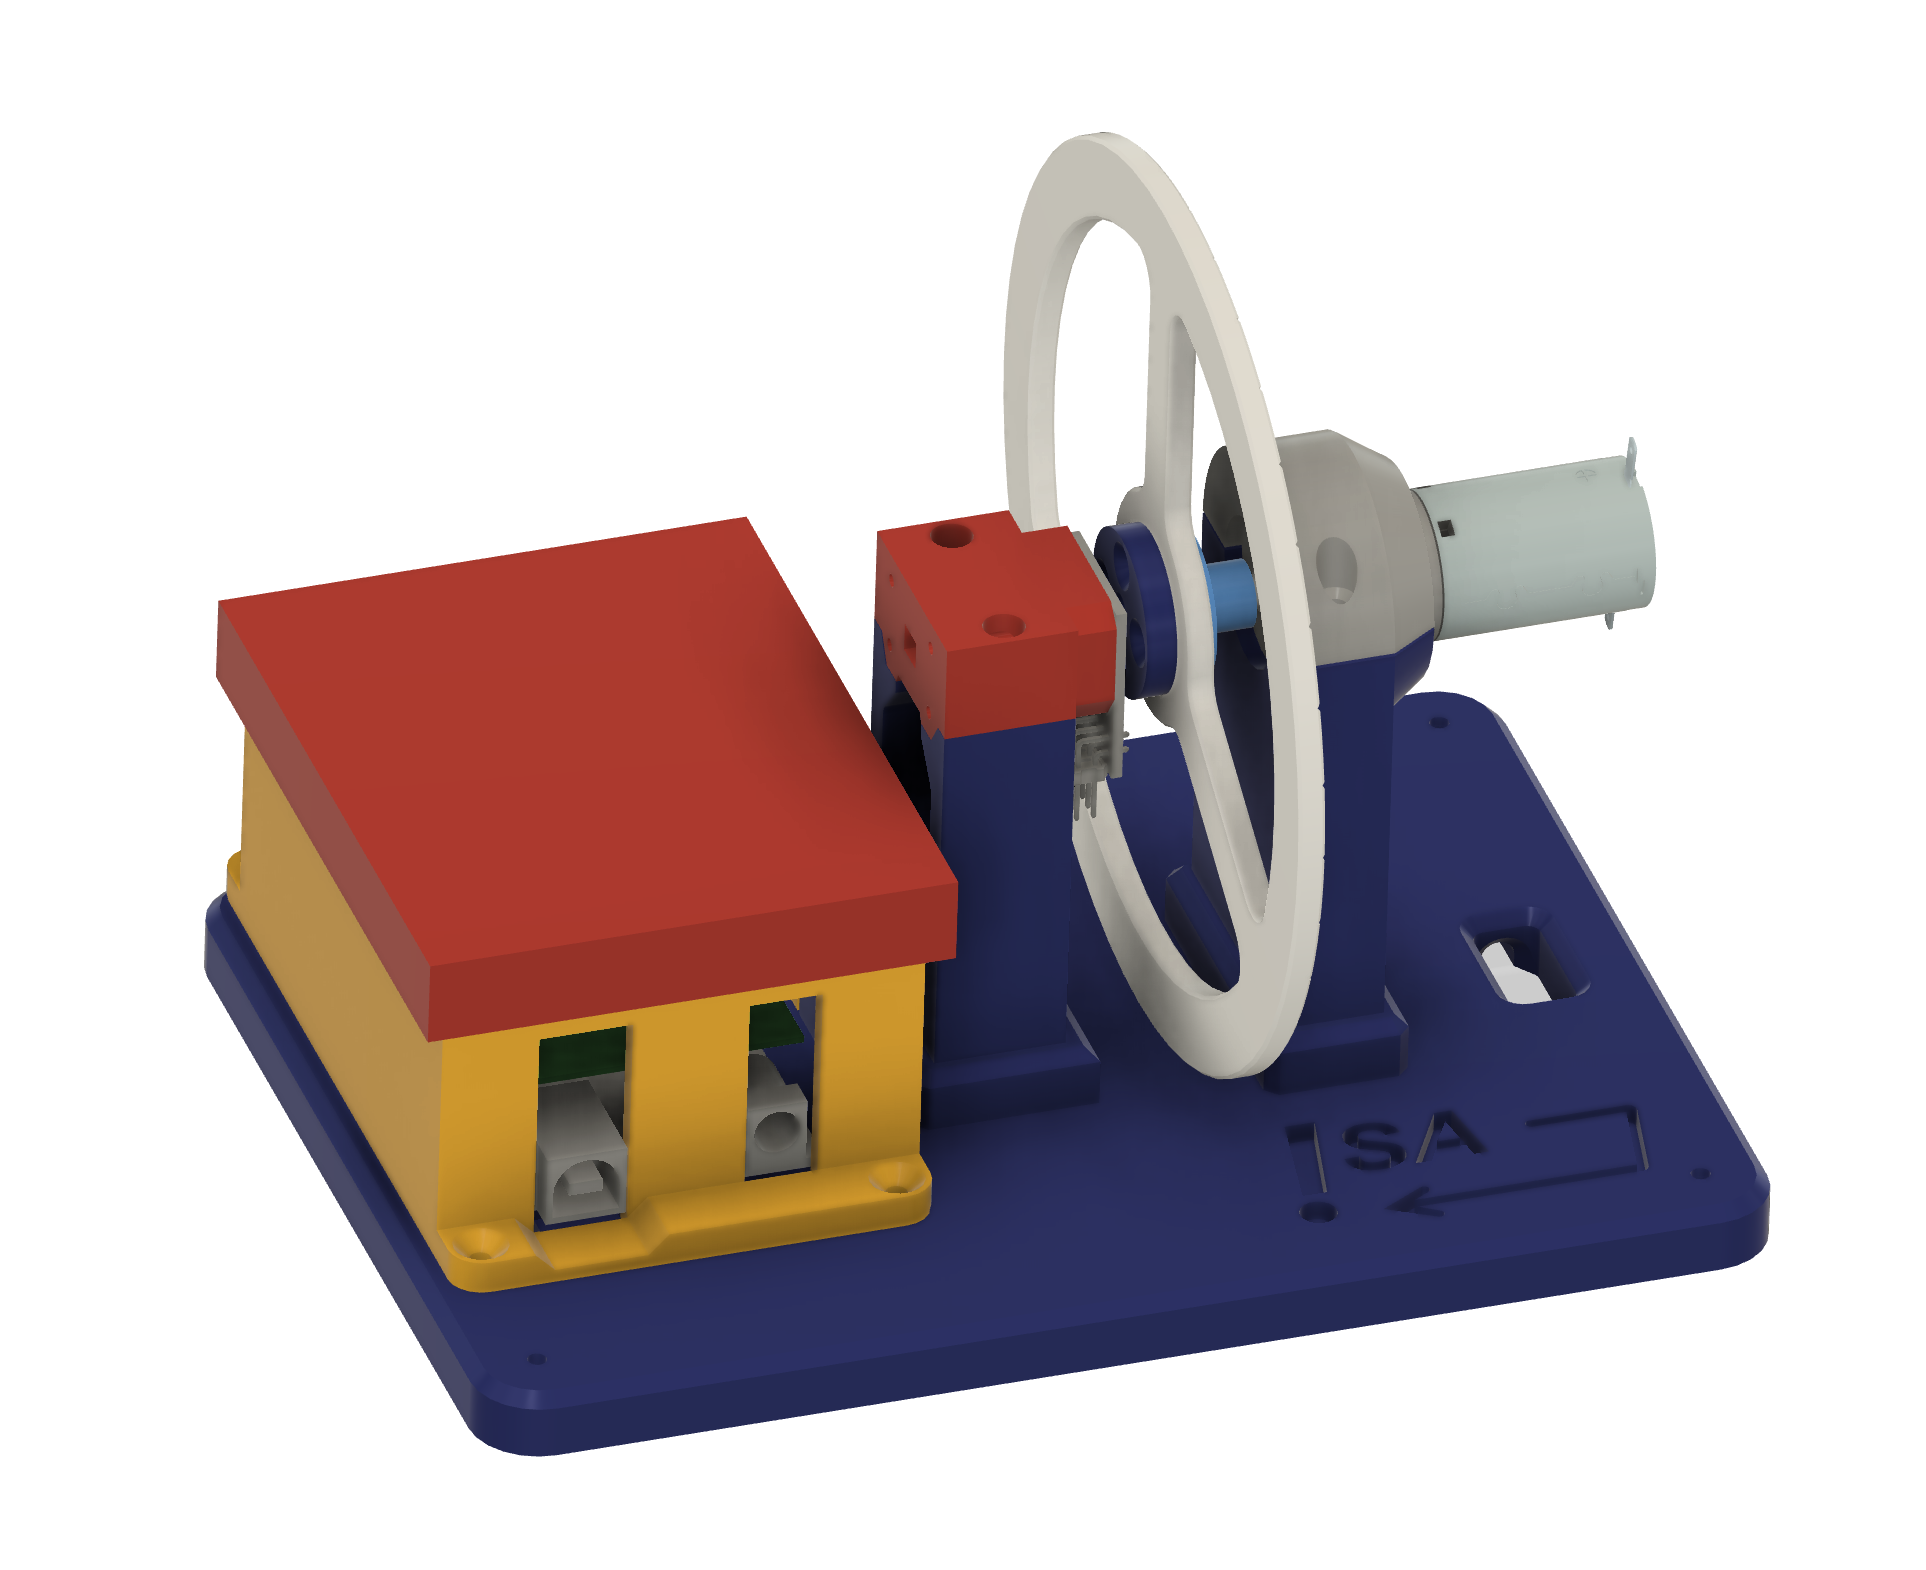
\includegraphics[width=\linewidth,height=2.3cm,keepaspectratio]{../images/equipo_render.png}
\end{minipage}\par
\smallskip\hrule\medskip

\textbf{Cuándo utilizar esta guía.} Solo para preparar un Arduino nuevo, sustituir la placa o actualizar el firmware. Si el equipo ya funciona, ve directamente a \texttt{manual\_usuario\_isa.pdf}. La carga queda guardada en Arduino al desconectarlo.

\section*{1. Preparar el ordenador}
Necesitas Arduino IDE 2.x, un Arduino UNO, un cable USB de datos y una copia del repositorio. MATLAB no interviene en la carga del firmware.

\textbf{Descarga primero los archivos.} Abre \href{https://github.com/DocMuerde/Motor-CC-Control-Lab}{github.com/DocMuerde/Motor-CC-Control-Lab}, pulsa \textbf{Code > Download ZIP} y descomprime el ZIP en una carpeta de tu ordenador.

\textbf{Alternativa con Git.} Si tienes Git, abre una terminal en la carpeta donde quieras guardar el proyecto y ejecuta:\par
{\small\ttfamily git clone https://github.com/DocMuerde/Motor-CC-Control-Lab.git}\par
En ambos casos, localiza la carpeta extraída o clonada: dentro está \texttt{firmware/arduino/main/main.ino}. No abras el archivo dentro del ZIP.

\textbf{Instala las bibliotecas de Arduino}
\begin{enumerate}
\item Abre Arduino IDE y su \textbf{Gestor de bibliotecas} (\emph{Library Manager}).
\item Busca e instala \textbf{AS5047P}, de Marginally Clever. Es la biblioteca utilizada por \texttt{\#include <AS5047P.h>}.
\item Busca e instala \textbf{MsTimer2}. Es la biblioteca utilizada por \texttt{\#include <MsTimer2.h>}. Las bibliotecas integradas del núcleo de Arduino se suministran con el entorno de la placa.
\end{enumerate}
Estas bibliotecas se necesitan en el ordenador que compila y carga el firmware; no en cada ordenador que utiliza el equipo desde MATLAB.

\clearpage
{\small\color{isa} Instalación del firmware · Arduino UNO}\par
\section*{2. Cargar el programa}
\begin{enumerate}
\item Deja desconectada la alimentación externa y conecta Arduino al ordenador por USB. Mantén libre el eje del motor. Cierra las simulaciones y cualquier programa que utilice el puerto serie.
\item En Arduino IDE, selecciona \textbf{Archivo > Abrir} y, dentro de la carpeta descargada o clonada, abre \texttt{firmware/arduino/main/main.ino}. Conserva el nombre de carpeta \texttt{main} y el nombre de archivo \texttt{main.ino}.
\item En \textbf{Herramientas > Placa}, selecciona \textbf{Arduino Uno} del paquete \textbf{Arduino AVR Boards}; instala ese paquete desde el Gestor de placas si falta.
\item En \textbf{Herramientas > Puerto}, selecciona el puerto del Arduino. Si dudas, desconecta y reconecta USB para identificar qué puerto aparece.
\item Pulsa \textbf{Verificar} para compilar. Si aparece un error de biblioteca no encontrada, comprueba las dos bibliotecas del apartado anterior.
\item Pulsa \textbf{Subir} y espera la confirmación de carga completada sin errores.
\end{enumerate}

\section*{3. Comprobar y pasar a MATLAB}
Como comprobación básica, puedes abrir el \textbf{Monitor Serie} a \textbf{115200 baudios}. El firmware envía paquetes binarios cada 10 ms: es normal ver símbolos ilegibles. Si el encoder no se inicializa, el firmware imprime un error de conexión SPI cada 5 s. La actividad serie por sí sola no verifica el accionamiento. No envíes comandos de texto.

\textbf{Cierra el Monitor Serie} para liberar el puerto. Sigue la guía rápida: abre el modelo de tu versión, haz doble clic en \textbf{Motor CC}, selecciona el puerto, pulsa \textbf{OK} y después \textbf{Run}. Comprueba las medidas de posición y velocidad en los Scopes.

\textbf{Si falla la carga:} revisa placa y puerto, cierra el Monitor Serie y MATLAB, y prueba otro cable USB de datos. Si no hay medidas, revisa las conexiones de shield y encoder con el equipo desconectado.

\textbf{Dependencias separadas:} para usar el equipo se necesita MATLAB con Simulink y únicamente \textbf{Instrument Control Toolbox} como toolbox adicional. Las bibliotecas de Arduino anteriores se utilizan solo para instalar o actualizar el firmware.

\end{document}
